%\vspace{-0.28cm}
%% \section{Perceptual Organization of the Image}

%% Our approach to organize the image is based on exploring various groupings of the image in a bottom up fashion. The output of this process is a set of possibly overlapping regions or object proposals. Traditionally the exploration or generation of diverse groupings has been treated as a combinatorial search problem in a discretized finite search space. For example, given a superpixel representation we can generate different object proposals by varying the levels of the region hierarchy or dendrogram, the number of superpixels at each level, and finally the cardinality of our merging step i.e. pairs, triplets, or quads. Each object proposal is then parameterized by one combination of these parameters and we can generate a set of object proposals by sweeping this parameter space. The same can be said for graph cut methods where the seed shape, seed location, seed size, and bias between energy terms are sufficiently discretized and swept to generate object proposals. In our work we deviate drastically from this ``regions by parameter sweeping'' approach by adopting a more structured and exhaustive methodology where by we look at the formation of a single object proposal not as merely a particular permutation of input parameters but rather as the result of a reorganization of an image, which is precisely captured by applying multiple transforms to our representation, or namely a transform sequence.  To generate multiple object proposals we explore many transform sequences spatially distributed across the image. In the following sections we illustrate the effects of a transform sequence, Section~\ref{sec:transform_seq}, on our representation and subsequently show how we can explore many such groupings efficiently, Section~\ref{sec:cgraph}. 

\section{Transform Sequences}
\label{sec:transform_seq}
%\vspace{-0.38cm}

A long-standing paradigm of computer vision and perceptual organization in understanding a scene with a number of objects is to assign an image region to each object, while the remaining information is organized as an attribute of these objects or the background. It is not surprising then that computer vision ground-truth databases often label regions corresponding to objects. Low-level vision cues of grouped regions and grouped edges in the form of curve fragments, however, differ from this ideal outcome precisely due to the four classes of degradations described earlier, namely, contour clutter, region clutter, contour gaps, and split regions, for each of which a corrective transform was designed. The path to reach this ideal outcome, therefore, is the judicious application of a set of transforms, Figure~\ref{fig:ma_transforms}, which are performed in sequence. In other words, an applicable transform is applied to the RECOIN representation and the process is repeated, leading to a \emph{fragment transform sequence}:  

\begin{definition}
A \emph{Fragment Transform Sequence (FTS)} is the application of a set of transforms, $\{T_1,T_2,...,T_N\}$, in sequence to the RECOIN representation of an image.
\label{def:fts}
\end{definition}


%% How can transforms organize the image into perceptually meaningful constructs? Borrowing cues from Gestalt psychologists, a complete object silhouette or region can be identified if the gaps in the silhouettes are completed and the clutter contours are removed, or alternatively, object sub-regions can be merged and clutter regions are removed. As was shown earlier, each of these operations individually are a fragment transform and a collection of them together is therefore a sequence of fragments transforms. Given our RECOIN representation the process of applying a sequence of transforms amounts to first detecting possible transformations, and then applying them, and finally repeating the process, Figure~\ref{fig:ma_transforms}. This repetitive procedure of detection and application of transforms we refer to as a \emph{fragment transform sequence}, Definition~\ref{def:fts}. 



%% \textcolor{red}{To Ben: Maybe this subsequence paragraph should be moved somewhere else} The idea of perceptual organization being expressed in the language of applying a sequence of symmetry (shock graph) transforms was proposed by~\cite{Johannes:POCV2001}. This theoretical work showed how, Figure~\ref{fig:ma_transforms}, a manual selected set of operations, completing a gap and removing a contour, could be utilized to organize a contour map. However, that work did not show how these sequences affect the image, and secondly did not propose a computational framework for detection or efficient ways for recomputing the shock graph at each step of the process. The work of Tamrakar \etal~\cite{Tamrakar:Kimia:POCV04} extended this prior work to show how contour based transforms could affect the image, but did not propose a computational framework for how to do it. 

\begin{figure}[ht]
\center
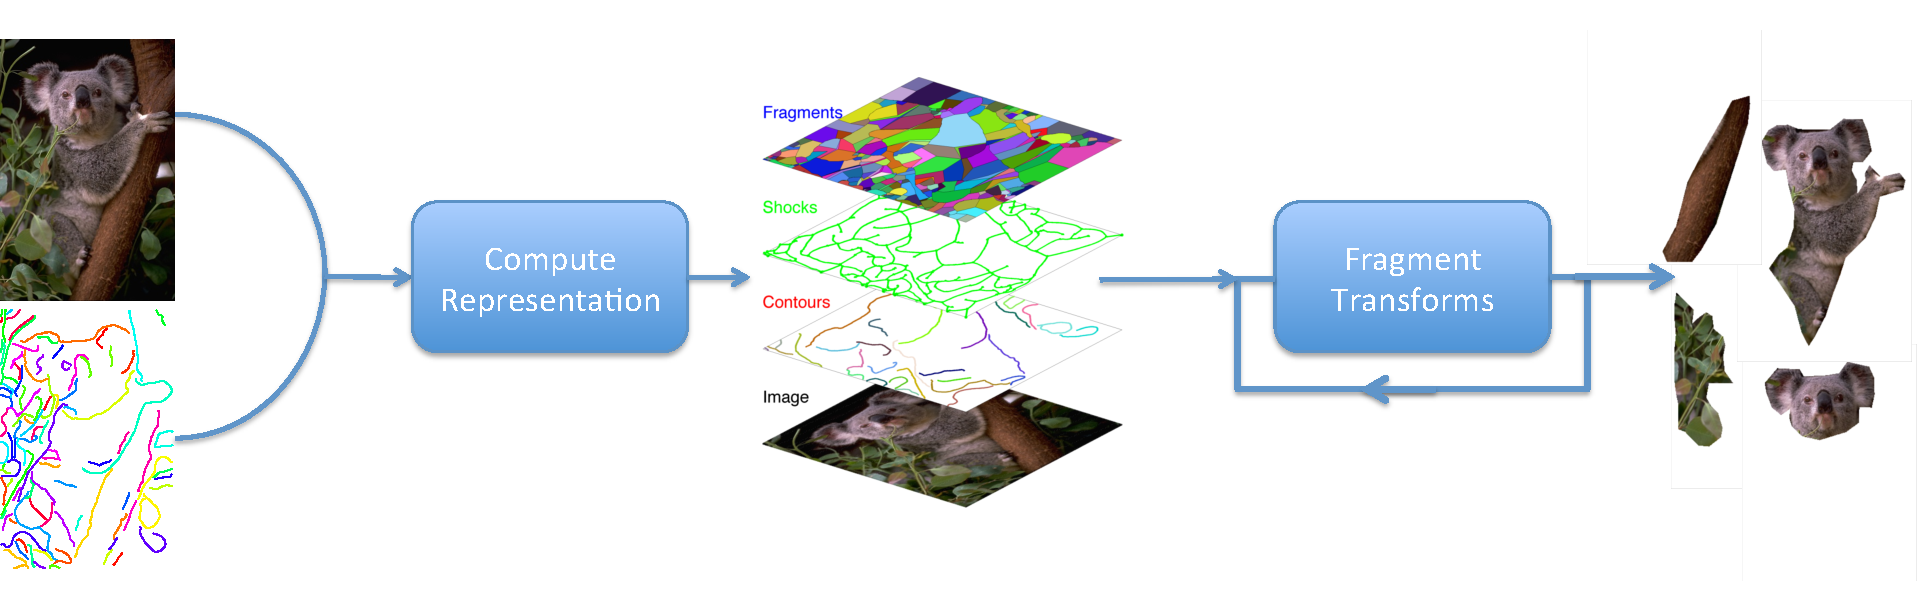
\includegraphics[width=0.8\textwidth]{figs/flowchart.pdf}
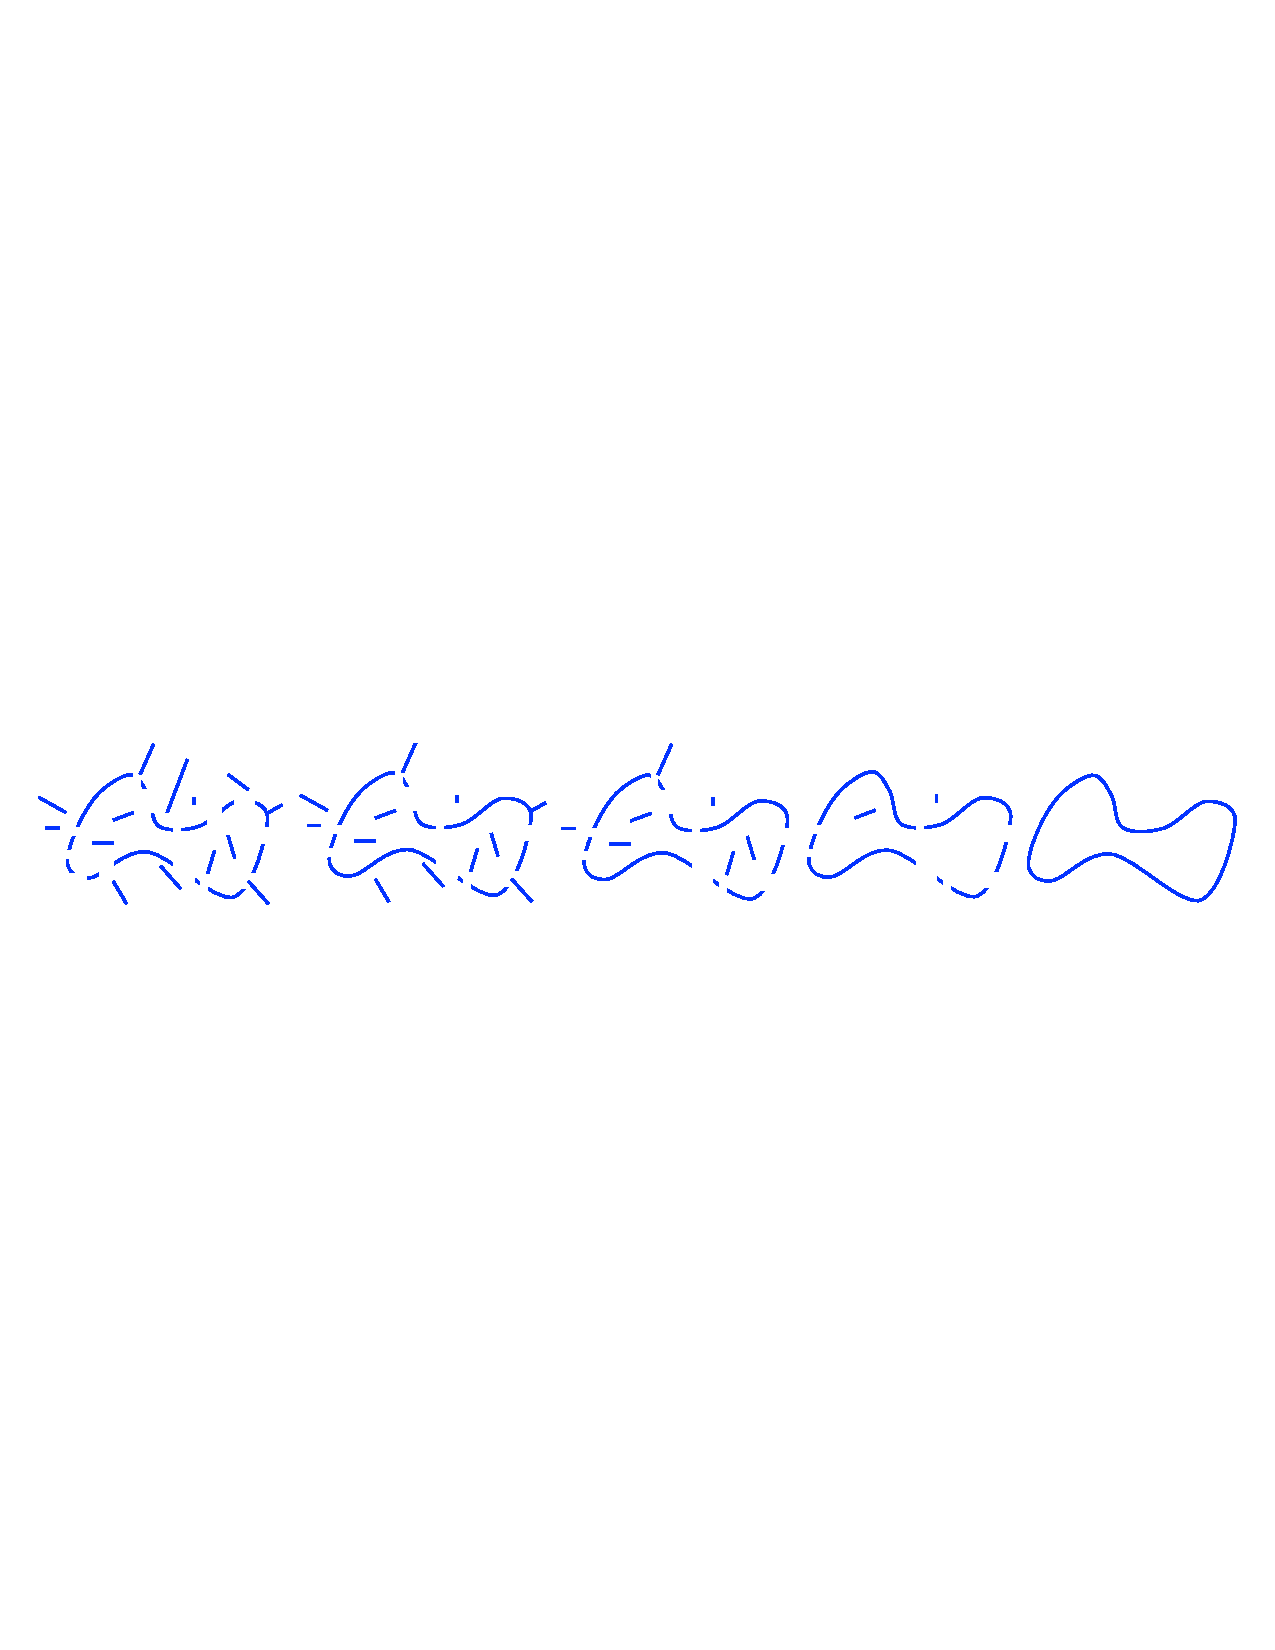
\includegraphics[width=0.8\textwidth]{figs/pocv_sequence.pdf}
\caption{A high level abstraction of our approach. In this view, our representation serves as a state of the image as it is, and transforms affect this state. This transform loop hopefully aims to lead to a more organized representation forming object parts and proposals. The bottom row shows how a set of contours becomes more regular through one particular transform sequence.} 
\label{fig:ma_transforms}
\end{figure}

%% \begin{figure*}[ht]
%% \centering
%% \setlength{\tabcolsep}{1pt}
%% \begin{tabular}{cccc}
%% a) Initial State & $Seq_1$: Apply $G_1$ & $Seq_1$: Apply $G_1,L_1$  & $Seq_1$: Apply $G_1,L_1,G_2$\\
 
%% 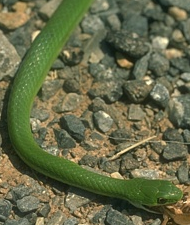
\includegraphics[width=0.24\textwidth]{figs/cropped_snake.png}&
%% 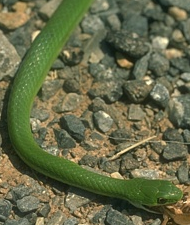
\includegraphics[width=0.24\textwidth]{figs/cropped_snake.png}&
%% \multicolumn{2}{c}{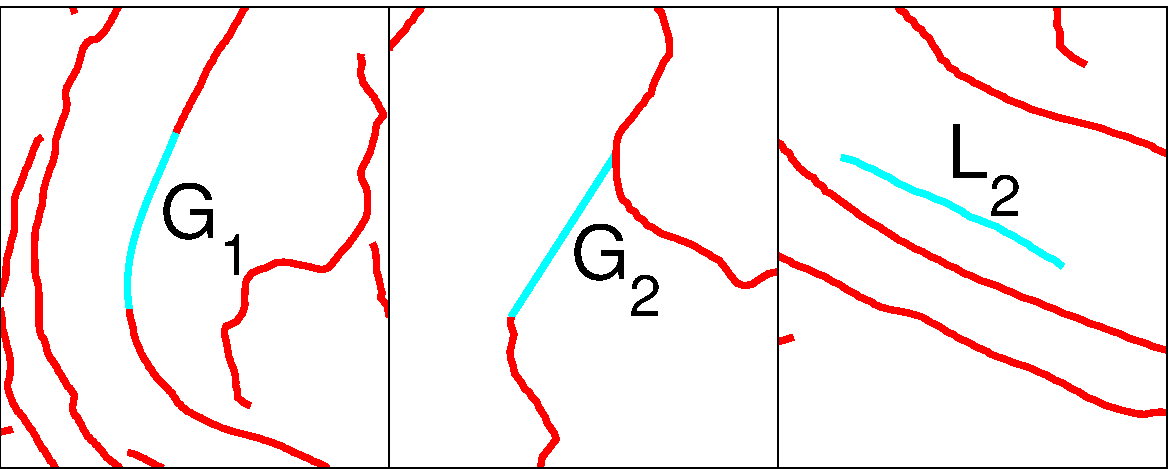
\includegraphics[width=0.24\textwidth]{figs/zoomin_gaps.pdf}}\\

%% 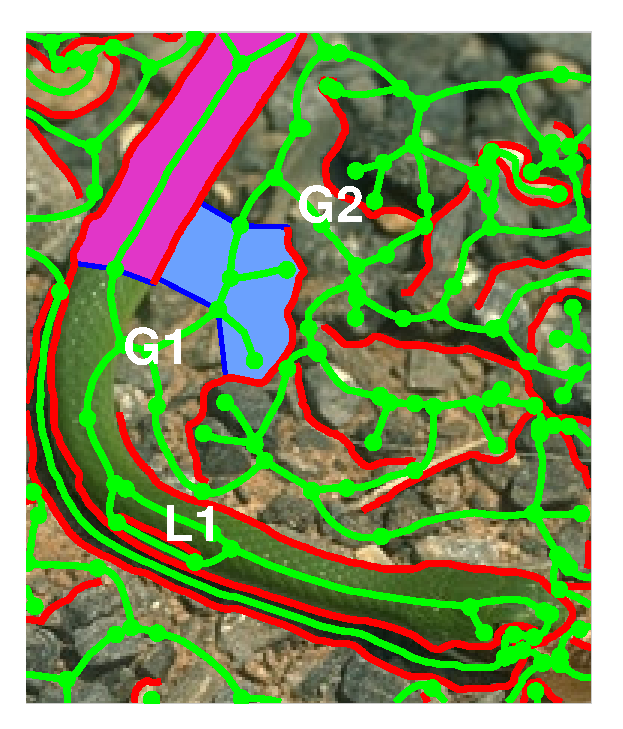
\includegraphics[width=0.24\textwidth]{figs/snake_start.pdf}&
%% 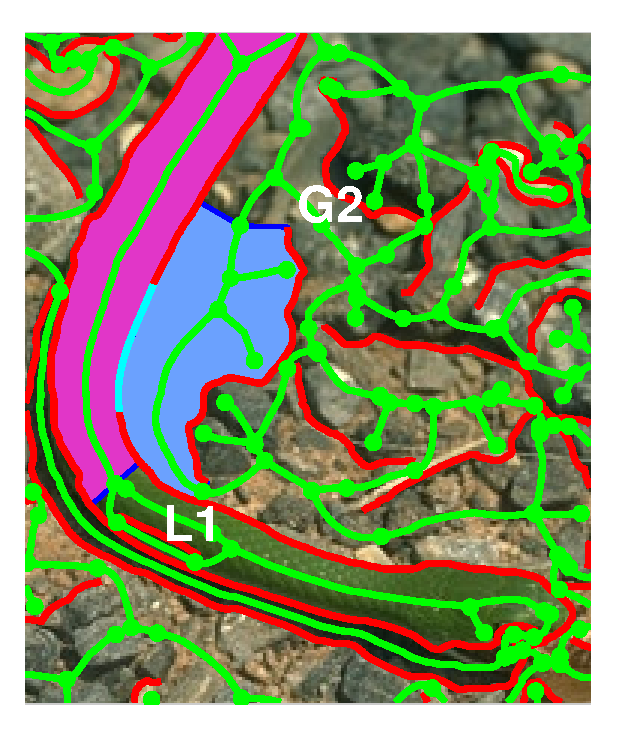
\includegraphics[width=0.24\textwidth]{figs/snake_t2.pdf}&
%% 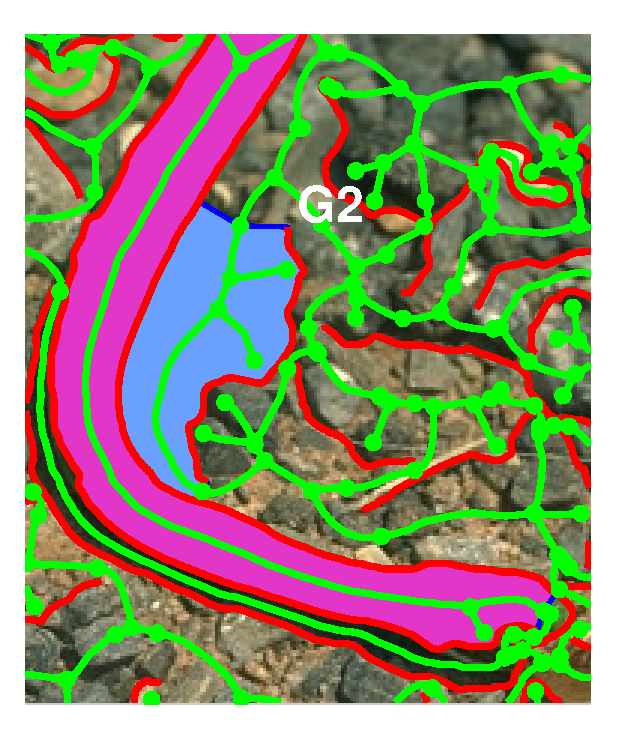
\includegraphics[width=0.24\textwidth]{figs/snake_t3.pdf}&
%% 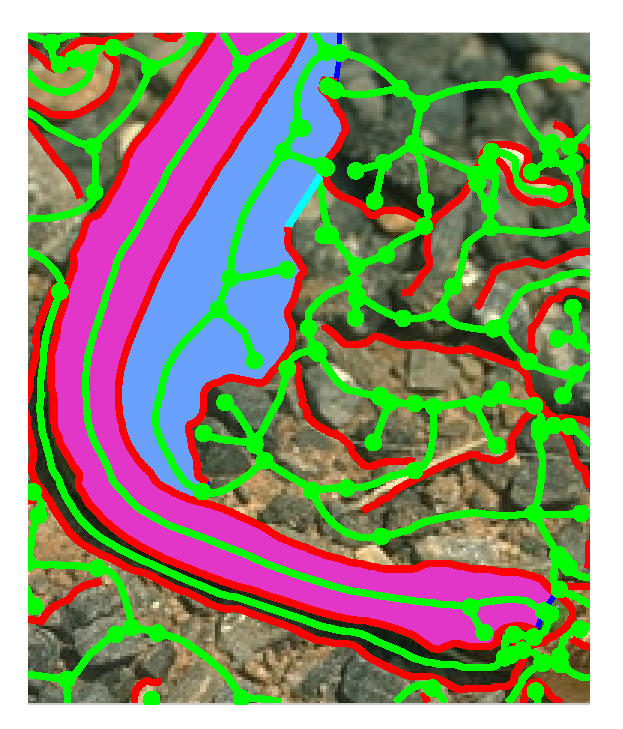
\includegraphics[width=0.24\textwidth]{figs/snake_t4.pdf}\\
%% %% 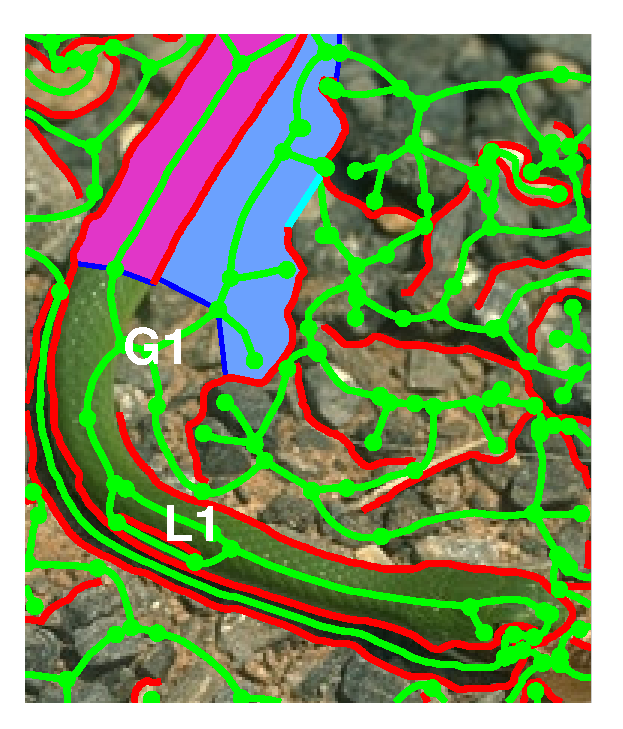
\includegraphics[width=0.24\textwidth]{figs/snake_t5.pdf}&
%% %% 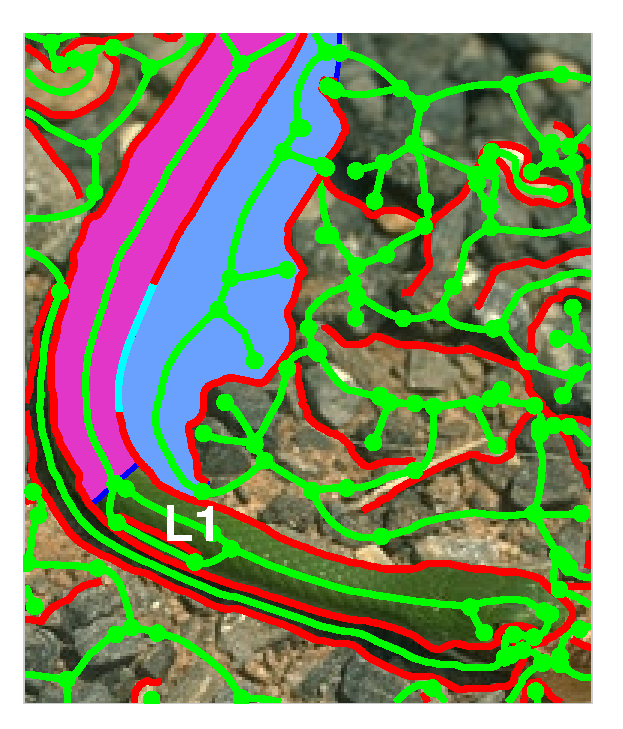
\includegraphics[width=0.24\textwidth]{figs/snake_t6.pdf}&
%% %% 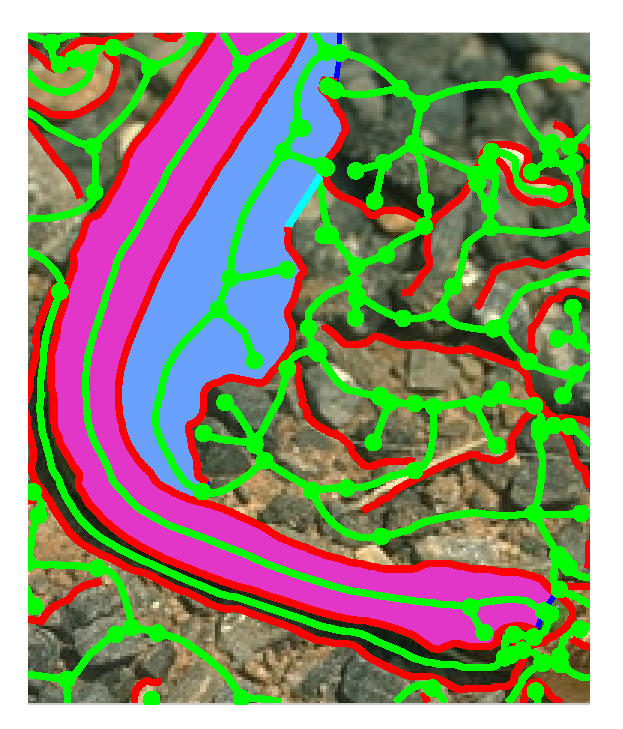
\includegraphics[width=0.24\textwidth]{figs/snake_t4.pdf}\\
%% \end{tabular}
%% 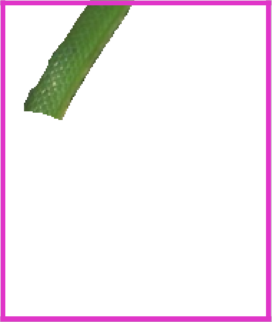
\includegraphics[width=0.12\textwidth]{figs/snake_t1.png}
%% 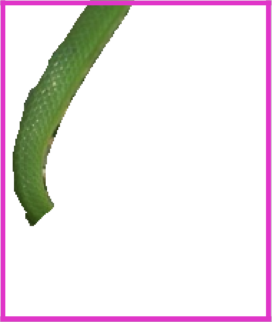
\includegraphics[width=0.12\textwidth]{figs/snake_t2.png}
%% 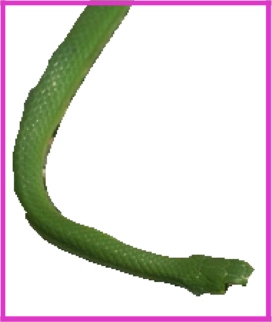
\includegraphics[width=0.12\textwidth]{figs/snake_t3.png}
%% 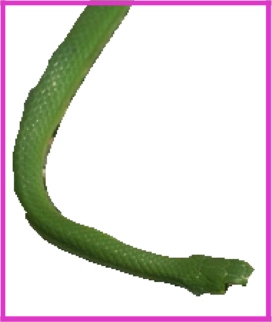
\includegraphics[width=0.12\textwidth]{figs/snake_t3.png}
%% 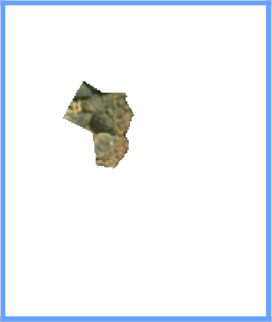
\includegraphics[width=0.12\textwidth]{figs/bg_t1.png}
%% 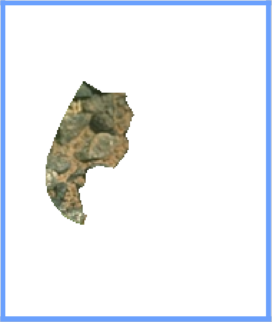
\includegraphics[width=0.12\textwidth]{figs/bg_t2.png}
%% 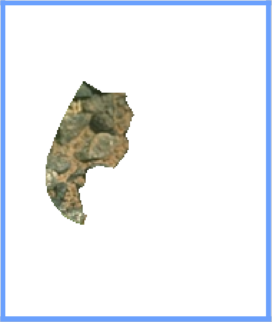
\includegraphics[width=0.12\textwidth]{figs/bg_t2.png}
%% 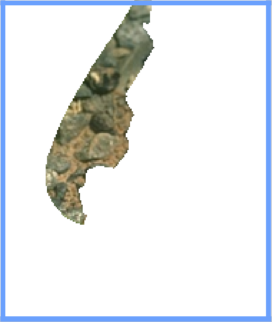
\includegraphics[width=0.12\textwidth]{figs/bg_t4.png}
%% \caption{A local area of our representation augmented with the location of transforms found during the detection process. $G_1$ and $G_2$ represent insertion of contour transforms, and $L_1$ represents a removal of a contour under consideration. For clarity sake, not all applicable transforms are shown and only two medial visual fragments are highlighted. We can organize this ``initial state'' by two sequences, represented as the first two rows of this figure. The top row represents the application of $G_1$ (completion curve in \textcolor{cyan}{cyan}) followed by $L_1$ and finally the transversal completion $G_2$ (completion curve in \textcolor{cyan}{cyan}) finishing the sequence $G_1 \rightarrow L_1 \rightarrow G_2$. The second row depicts the sequence $G_2 \rightarrow G_1 \rightarrow L_1$. The set of all object proposals from both sequences can be seen in the bottom row of the figure, color coded to match the representative fragments as seen above. }
%% \label{fig:snake_seq}
%% \end{figure*}

\begin{figure*}[p]
\centering
\setlength{\tabcolsep}{1pt}
\begin{tabular}{cccc}
%% a) Image/Initial State & $Seq_1$: Apply $G_1$ & $Seq_1$: Apply $G_1,L_1$  & $Seq_1$: Apply $G_1,L_1,G_2$\\
\multirow{3}{*}[1.63in]{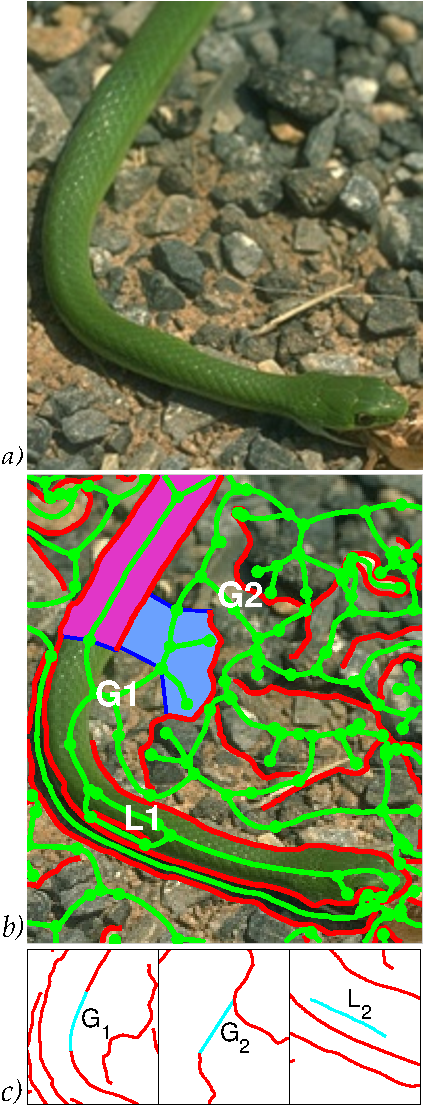
\includegraphics[height=0.60\textwidth]{figs/snake_cs_start3.pdf}}&
{\footnotesize\textit{\textcolor{black}{d)}}}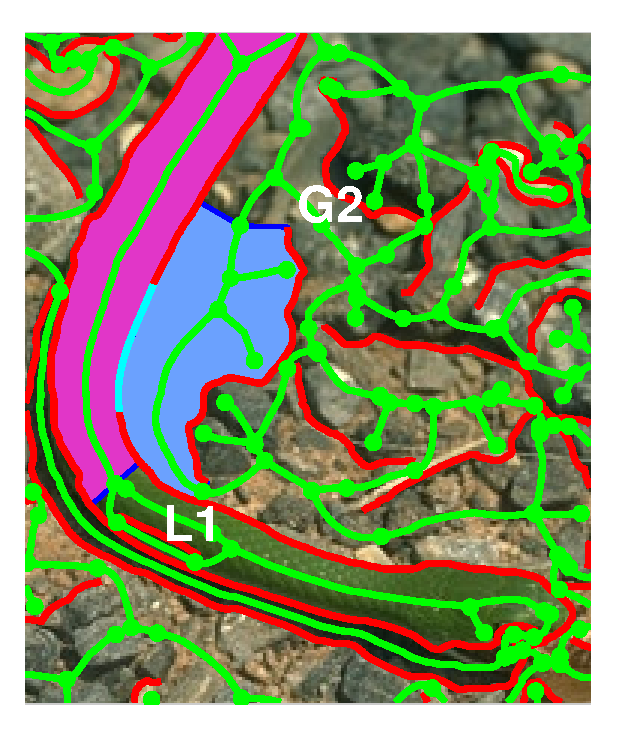
\includegraphics[width=0.2465\textwidth]{figs/snake_t2.pdf}&
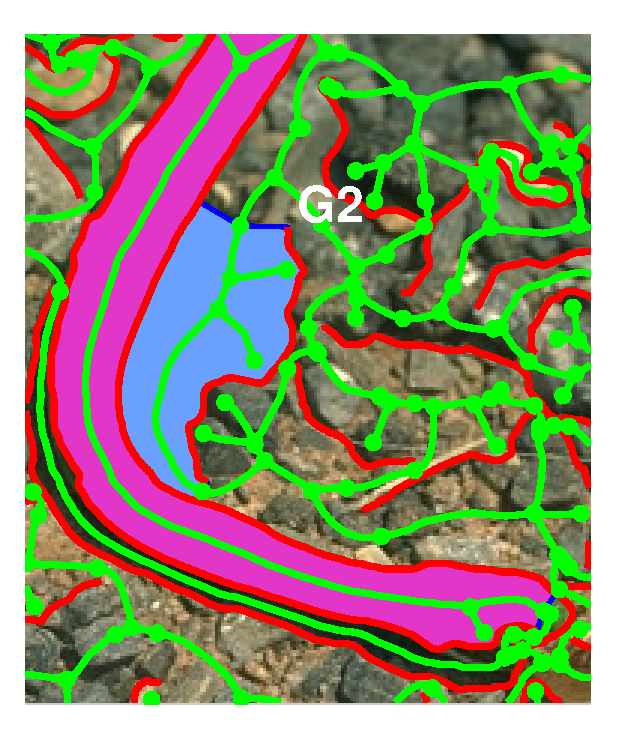
\includegraphics[width=0.2465\textwidth]{figs/snake_t3.pdf}&
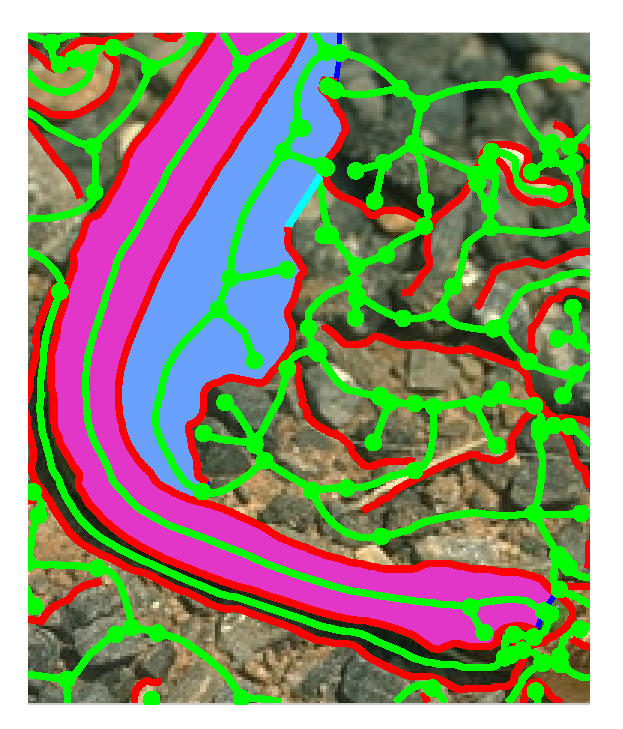
\includegraphics[width=0.2465\textwidth]{figs/snake_t4.pdf}\\
%% & $Seq_2$: Apply $G_2$ & $Seq_2$: Apply $G_2,G_1$  & $Seq_2$: Apply $G_2,G_1,L_1$\\
&
{\footnotesize\textit{\textcolor{black}{e)}}}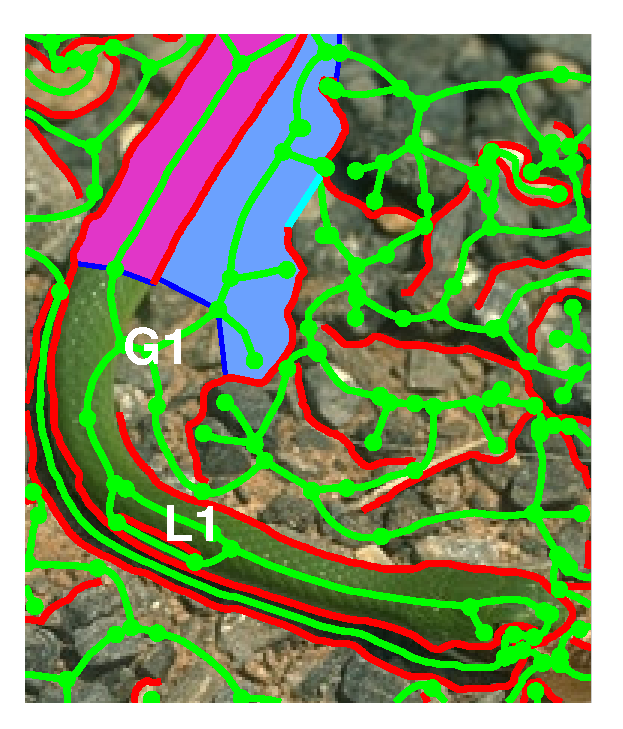
\includegraphics[width=0.2465\textwidth]{figs/snake_t5.pdf}&
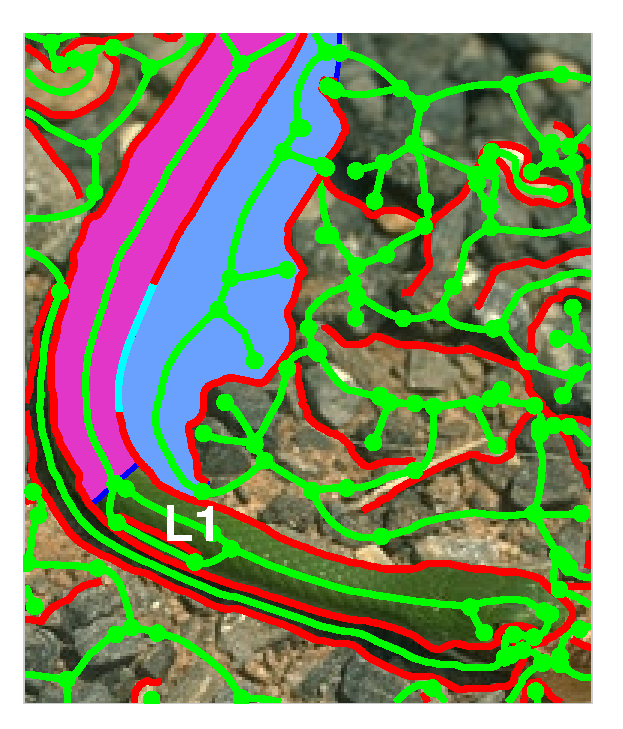
\includegraphics[width=0.2465\textwidth]{figs/snake_t6.pdf}&
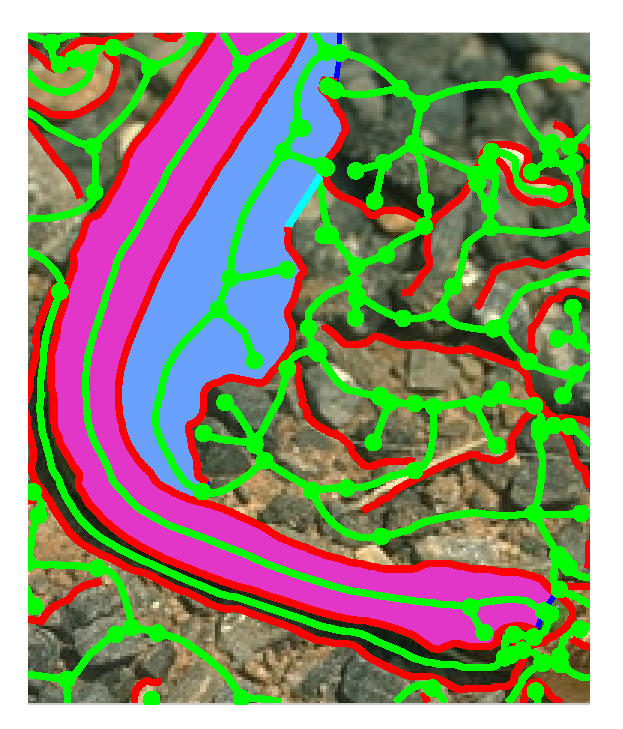
\includegraphics[width=0.2465\textwidth]{figs/snake_t4.pdf}\\
\end{tabular}
{\footnotesize\textit{\textcolor{black}{f)}}}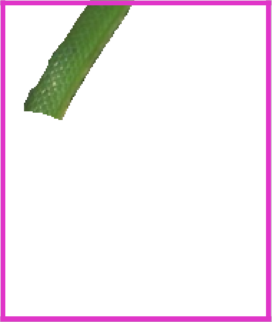
\includegraphics[width=0.118\textwidth]{figs/snake_t1.png}
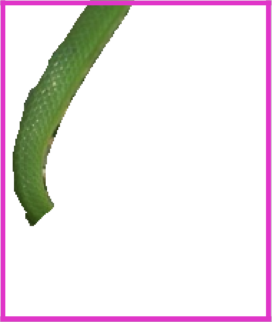
\includegraphics[width=0.118\textwidth]{figs/snake_t2.png}
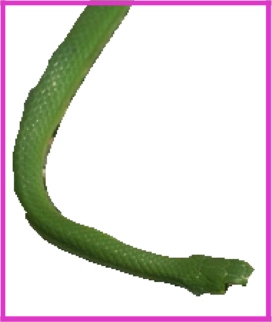
\includegraphics[width=0.118\textwidth]{figs/snake_t3.png}
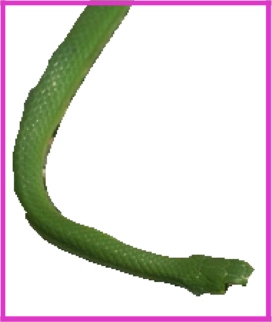
\includegraphics[width=0.118\textwidth]{figs/snake_t3.png}
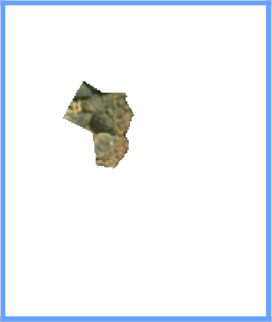
\includegraphics[width=0.118\textwidth]{figs/bg_t1.png}
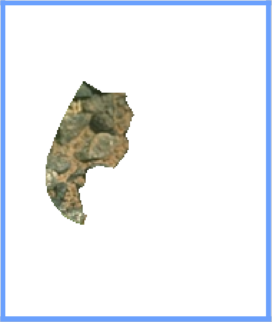
\includegraphics[width=0.118\textwidth]{figs/bg_t2.png}
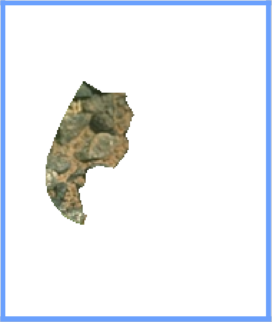
\includegraphics[width=0.118\textwidth]{figs/bg_t2.png}
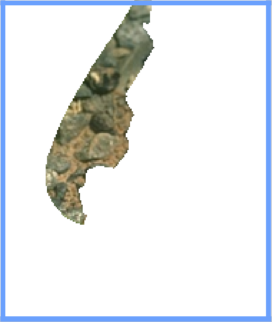
\includegraphics[width=0.118\textwidth]{figs/bg_t4.png}

%% 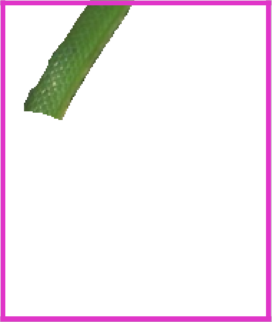
\includegraphics[width=0.16\textwidth]{figs/snake_t1.png}
%% 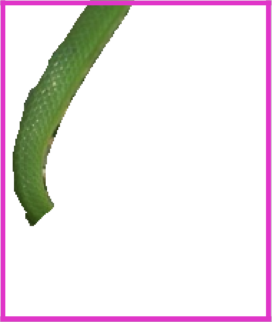
\includegraphics[width=0.16\textwidth]{figs/snake_t2.png}
%% 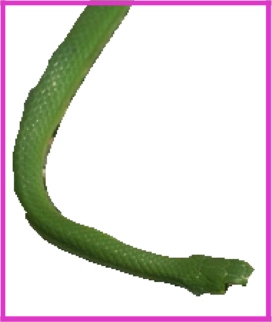
\includegraphics[width=0.16\textwidth]{figs/snake_t3.png}
%% 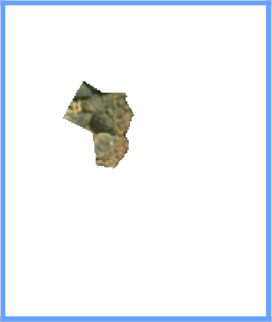
\includegraphics[width=0.16\textwidth]{figs/bg_t1.png}
%% 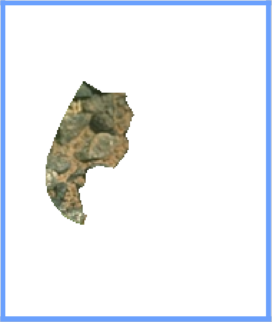
\includegraphics[width=0.16\textwidth]{figs/bg_t2.png}
%% 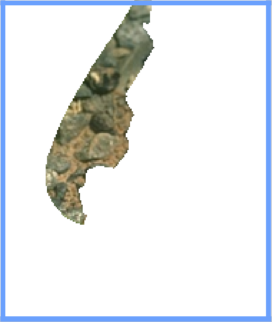
\includegraphics[width=0.16\textwidth]{figs/bg_t4.png}
\caption{An illustration of the effect of two transform sequences. (a) Original image of a green snake on a gray background. (b) Contours are shown in red and shocks in green. Observe how the formation of the snake region is interrupted by a missing contour, marked by $G_1$ and clutter contour marked by $L_1$. The gap $G_2$ is unrelated to the snake. For clarity, not all applicable transforms and medial visual fragments are highlighted. (c) Each gap can be completed by a transform, $G_1$ and $G_2$, and the clutter contour can be removed by the appropriate transformation. (d) The result of applying the sequence $(G_1,L_1,G_2)$ as compared to the transform sequence $(G_2,G_1,L_1)$ shown in (e). (f) The set of all object proposals generated from these two sequences. }
%% \caption{A local area of our representation augmented with the location of transforms found during the detection process. $G_1$ and $G_2$ represent insertion of contour transforms, and $L_1$ represents a removal of a contour under consideration. For clarity sake, not all applicable transforms are shown and only two medial visual fragments are highlighted. We can organize this ``initial state'' by two sequences, represented as the first two rows of this figure. The top row represents the application of $G_1$ (completion curve in \textcolor{cyan}{cyan}) followed by $L_1$ and finally the transversal completion $G_2$ (completion curve in \textcolor{cyan}{cyan}) finishing the sequence $G_1 \rightarrow L_1 \rightarrow G_2$. The second row depicts the sequence $G_2 \rightarrow G_1 \rightarrow L_1$. The set of all object proposals from both sequences can be seen in the bottom row of the figure, color coded to match the representative fragments as seen above. }
\label{fig:snake_seq}
\end{figure*}

The immediate and key question is how to form a FTS from among the many applicable transforms. A simple example in Figure~\ref{fig:snake_seq} illustrates this process: the silhouette of the green snake on gray rocks is interrupted by a contour gap marked as ``$G_1$'', and a clutter contour, marked as ``$L_1$'', interferes with the formation of the snake region as a single fragment, Figure~\ref{fig:snake_seq}\textcolor{red}{(b,c)}. A fragment transform sequence that includes $G_1$ and $L_1$, in either order, leads to the desirable outcome of the snake region as a fragment. However, there are numerous other applicable transforms, most of which do not interfere with the formation of the snake fragment and are irrelevant to it, \eg, the gap in a background contour marked as ``$G_2$'' (other transforms are not shown for clarity). The application of two transform sequences $(G_1,L_1,G_2)$ and $(G_2,G_1,L_1)$ is shown in Figure~\ref{fig:snake_seq}\textcolor{red}{(d,e)} respectively. Note that while the final outcome of the two FTS are the same, the intermediate organizations are not. Since apriori it is not clear where an object forms in the application of a transform sequence, all intervening formed fragments are retained as potential object fragments, or object proposals, as shown in Figure~\ref{fig:snake_seq}\textcolor{red}{(f)}. 



%% The top row shows that, in this case, the FTS $(G_1 \rightarrow L_1 \rightarrow G_2)$ leads to the same outcome as $(G_2 \rightarrow G_1 \rightarrow L_1)$ both containing the snake fragment. 

%% We illustrate some simple examples of how \emph{fragment transform sequences} perceptually organize our RECOIN representation, and explore properties of them. Figure~\ref{fig:snake_seq} illustrates how our representation changes by way of a manually selected transformation sequence. The initial picture depicts the state of our representation after detecting a set of possible transforms. $Seq_1$, top row of Figure~\ref{fig:snake_seq}, illustrates the process of applying each of these detected transforms in a particular order. Each subsequent subfigure in $Seq_1$ is identical to earlier figures depicting the output of a single transformation. When viewed as a sequence, rather than individual snapshots, we see that the effect of this set of transforms has resulted in the formation of larger regions \ie  region grouping. The final set of object proposals that would be output as a byproduct of this exploration can be seen in the bottom row of Figure~\ref{fig:snake_seq}. 

Transform sequences with identical outcomes arise when the individual transforms are independent in that each transform does not affect the applicability and outcome of another transform. Then, any permutation of transforms leads to the same result. In other cases, however, the application of a transform can affect the applicability or the outcome of another transform. Consider another simple example of a white mushroom on a background of moss and green leaves, Figure~\ref{fig:mushroom_seq}, to illustrate this point. There are two gaps, marked as ``$G_2$'' and ``$G_3$'', Figure~\ref{fig:mushroom_seq}\textcolor{red}{(b,c)}, which disconnect the mushroom from its stem. The application of a sequence of $G_2$ and $G_3$ contour completion transforms, in either order, completes these gaps. However, the stem and the head of the mushroom remain disconnected because the contour ``$L_1$'', freshly identified after the application of $G_2$ and $G_3$ transforms, separates them. The application of a contour clutter removal transform completes the mushroom fragment, Figure~\ref{fig:mushroom_seq}\textcolor{red}{(d)}. A different sequence, starting with $G_1$, Figure~\ref{fig:mushroom_seq}\textcolor{red}{(e)}, completes the stem, but also removes $G_2$ and $G_3$ as applicable transforms. This sequence of one transform ($G_1$) completes the mushroom stem with object proposals shown from both sequences in Figure~\ref{fig:mushroom_seq}\textcolor{red}{(f)}. 

%% The second row of Figure~\ref{fig:mushroom_seq} explores a different sequence: here a third gap identified as ``$G_1$'' is completed through the application of a contour completion transform. Observe that executing this one-length FTS removes the applicability of completing $G_2$ and $G_3$.

Figure~\ref{fig:mushroom_seq} illustrates how the application of a transform sequence can \emph{(i)} can introduce a new applicable transform and \emph{(ii)} remove applicable transforms. Thus, the formation of transform sequences is dynamic.  Finally, a much more challenging image in Figure~\ref{fig:tiger_seq} illustrates the power of our transformations to organize a recognizable object proposal. This particular example does not show all the steps, but in general a ten to fifteen length transform sequence is needed to recover an object in a complex scene.
 
These examples illustrate how \emph{fragment transform sequences} can lead to meaningful groupings, however, what is not clear is whether and how these appropriate transform sequences can be selected from an undoubtedly large search space of transform sequences. Issues of transform independence, redundancy of sequences, and transform dynamics as illustrated in Figure~\ref{fig:snake_seq} and Figure~\ref{fig:mushroom_seq} play a significant role in understanding whether it is practical to search this space, as discussed next. 
  

%% Another possibility for organizing this local area of the image, could be as shown in $Seq_2$, where we have applied $G_2$ first, $G_1$ second, and finally $L_1$. If we compare individual steps between the two sequences we can see that the transformed representations differ, but the final representations are identical. Even more the set of object proposals produced by each are equivalent just generated at different steps during their respective sequences. In fact, any other permutation of these three transforms, $L_1 \rightarrow G_1 \rightarrow G_2$ for example, would lead to the same final transformed state. This does {\bf not} imply that subsequences produce equivalent representations or object proposals, but only that the final representation after applying same length sequences, in this case three, are equivalent. Another way to state this, is that there are many redundant length three sequences within our representation. More generally, the application of any permutation of a $N$ length transformation sequence, will lead to identical representations. This property, however, assumes that all transforms are independent, \ie the application of one transform does not nullify the application of any other transform. We show in subsequent examples where this assumption does not hold. 


 

%% \begin{figure}[ht]
%% \centering
%% \setlength{\tabcolsep}{1pt}
%% \begin{tabular}{cc}
%% a) Initial State & b) Apply $G_1$\\
%% 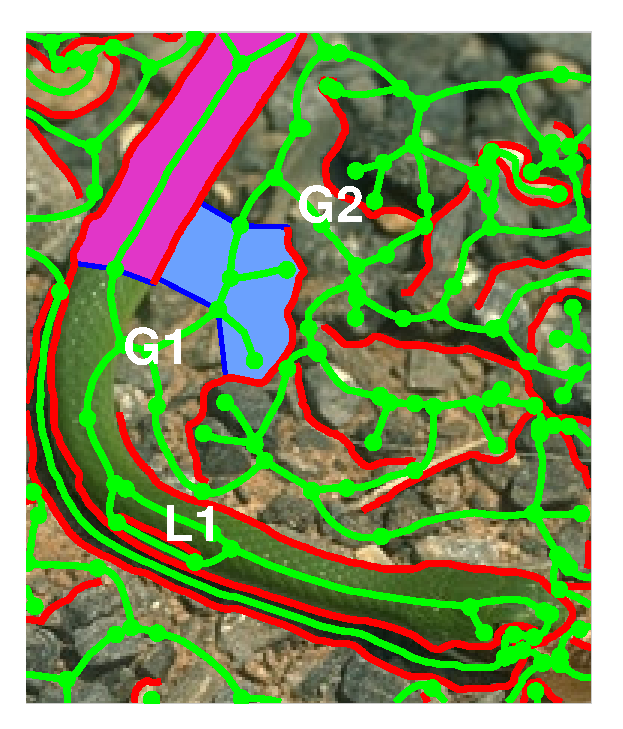
\includegraphics[width=0.24\textwidth]{figs/snake_start.pdf}&
%% 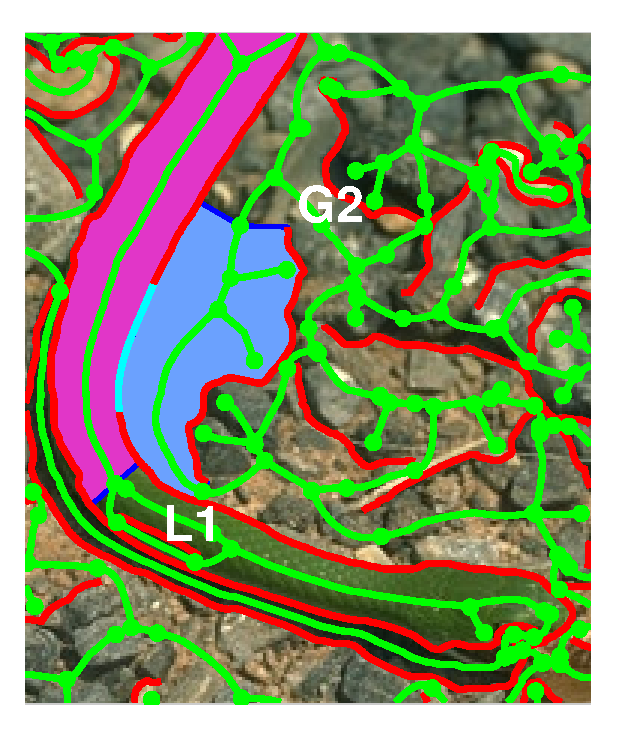
\includegraphics[width=0.24\textwidth]{figs/snake_t2.pdf}\\
%% c) Apply $G_1,L_1$ & d) Apply $G_1,L_1,G_2$\\
%% 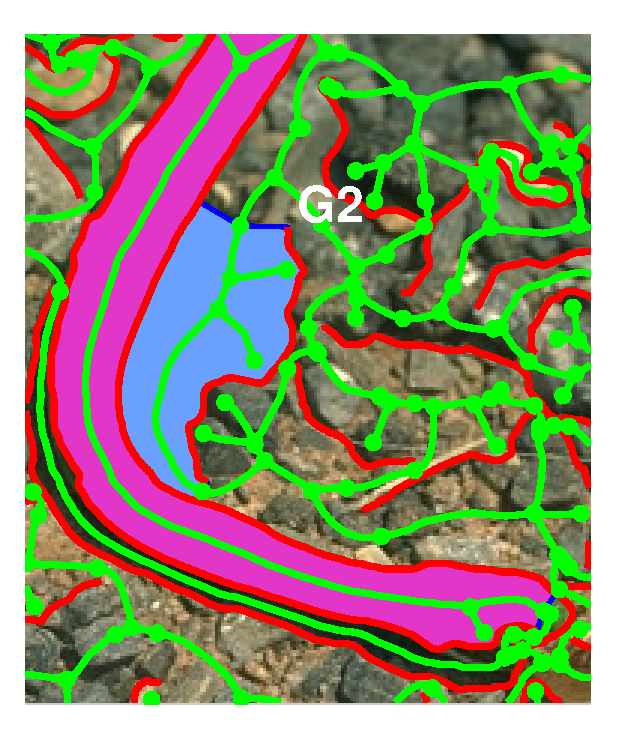
\includegraphics[width=0.24\textwidth]{figs/snake_t3.pdf}&
%% 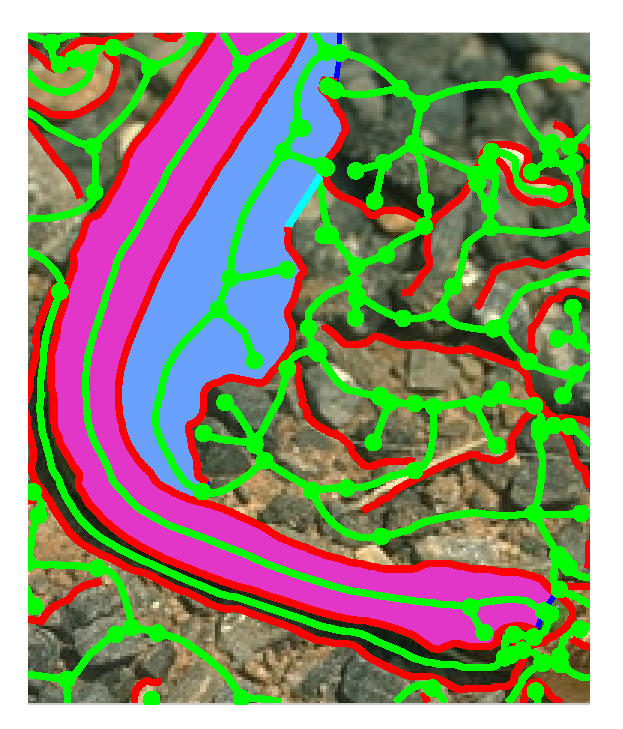
\includegraphics[width=0.24\textwidth]{figs/snake_t4.pdf}\\
%% \end{tabular}
%% \caption{a) A local area of our representation augmented with the location of transforms found during the detection process. $G_1$ and $G_2$ represent insertion of contour transforms, and $L_1$ represents a removal of a contour under considerations. For clarity sake, not all applicable transforms are shown and only two medial visual fragments are highlighted. b) The application of $G_1$ (completion curve in \textcolor{cyan}{cyan}) and the next transformation under consideration $L_1$. c) Application of removal of contour, $L_2$ and the next transformation under consideration, $G_2$. d) The final picture after transversal completion $G_2$ (completion curve in \textcolor{cyan}{cyan}) has been applied finishing the sequence $G_1 \rightarrow L_1 \rightarrow G_2$. }
%% \label{fig:snake_seq}
%% \end{figure}

%% \begin{figure}[ht]
%% \centering
%% 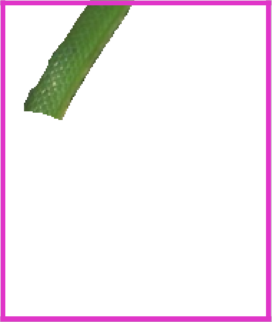
\includegraphics[width=0.15\textwidth]{figs/snake_t1.png}
%% 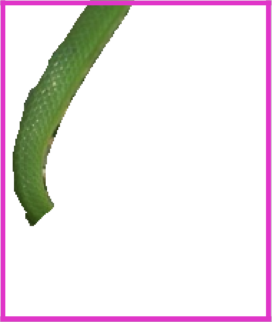
\includegraphics[width=0.15\textwidth]{figs/snake_t2.png}
%% 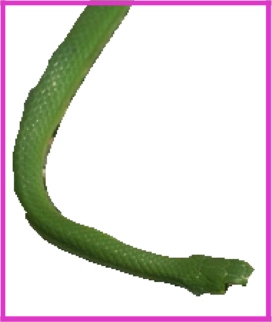
\includegraphics[width=0.15\textwidth]{figs/snake_t3.png}
%% 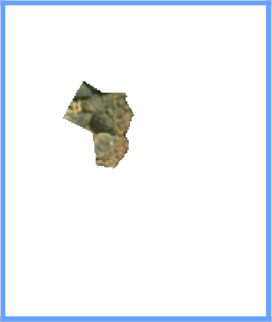
\includegraphics[width=0.15\textwidth]{figs/bg_t1.png}
%% 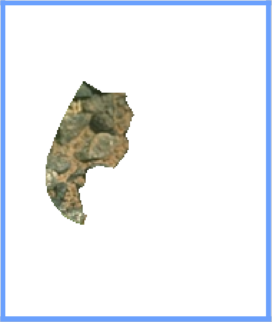
\includegraphics[width=0.15\textwidth]{figs/bg_t2.png}
%% \includegraphics[width=0.15\textwidth]{figs/bg_t4.png}
%% \caption{The output object proposals after exploring the sequence outlined in Figure~\ref{fig:snake_seq}. Notice the formation of pieces or parts of the green snake formed as a result of the transformations. }
%% \label{fig:snake_ops}
%% \end{figure}

\begin{figure*}[ht]
\centering
\setlength{\tabcolsep}{1pt}
\begin{tabular}{cccc}
%% a) Initial State & $Seq_1$: Apply $G_2$ & $Seq_1$: Apply $G_2,G_3$  & $Seq_1$: Apply $G_2,G_3,L_1$\\
 \multirow{3}{*}[1.7in]{\includegraphics[width=0.24\textwidth]{figs/mushroom_cs_start2.pdf}}&
{\footnotesize\textit{\textcolor{black}{d)}}}\includegraphics[width=0.242\textwidth]{figs/mushroom_t2.pdf}&
\includegraphics[width=0.242\textwidth]{figs/mushroom_t3.pdf}&
\includegraphics[width=0.242\textwidth]{figs/mushroom_t4.pdf}\\
%%& $Seq_2$: Apply $G_1$ &  &\\
&
{\footnotesize\textit{\textcolor{black}{e)}}}\includegraphics[width=0.242\textwidth]{figs/mushroom_t1.pdf}&
{\footnotesize\textit{\textcolor{black}{f)}}}\includegraphics[width=0.242\textwidth]{figs/mushroom_full_t4.png}&
\includegraphics[width=0.242\textwidth]{figs/mushroom_combine.png} \\
\end{tabular}
\caption{A transform can become inapplicable after the application of another transform. (a) Original image of a mushroom. (b) Three contour gaps are highlighted which can be completed by contour completion transforms, $G_1$,$G_2$, and $G_3$ as shown in (c). For clarity, not all applicable transforms and medial visual fragments are highlighted. (d) The transform sequence $(G_2,G_3,L_1)$ forms a full mushroom. However, the application of $G_1$, (e), renders transforms $G_2$ and $G_3$ inapplicable leading to a mushroom head and mushroom stem, separately. (f) The three object proposals which result.} 
%% \caption{A local area of our representation augmented with the location of transforms found during the detection process. $G_1$, $G_2$, and $G_3$ represent insertion of contour transforms under consideration. For clarity sake, not all applicable transforms are shown and only two medial visual fragments are highlighted.  We can organize this ``initial state'' by two sequences, represented as the first two rows of this figure. The top row represents the application of $G_2$ (completion curve in \textcolor{cyan}{cyan}) followed by $G_3$ (completion curve in \textcolor{cyan}{cyan}) and finally removing a piece of contour represented by $L_1$ thus finishing the sequence $G_2 \rightarrow G_3 \rightarrow L_1$. The second row depicts the sequence $G_1$. The set of all object proposals from both sequences can be seen in the bottom row of the figure.}
\label{fig:mushroom_seq}
\end{figure*}
 


%% \begin{figure}[ht]
%% \centering
%% \setlength{\tabcolsep}{1pt}
%% \begin{tabular}{cc}
%% a) Initial State & b) Apply $G_1$\\
%% \includegraphics[width=0.24\textwidth]{figs/mushroom_start.pdf}&
%% \includegraphics[width=0.24\textwidth]{figs/mushroom_t1.pdf}\\
%% \end{tabular}
%% \caption{a) A local area of our representation augmented with the location of transforms found during the detection process. $G_1$, represents insertion of contour transforms. For clarity sake, not all applicable transforms are shown and only two medial visual fragments are highlighted. b) The application of $G_1$ (completion curve in \textcolor{cyan}{cyan}). This sequence of length 1 invalidates all other transforms under consideration.  }
%% \label{fig:mushroom_seq_a}
%% \end{figure}

%% \begin{figure}[ht]
%% \centering
%% \setlength{\tabcolsep}{1pt}
%% \begin{tabular}{cc}
%% a) Initial State & b) Apply $G_2$\\
%% \includegraphics[width=0.24\textwidth]{figs/mushroom_start.pdf}&
%% \includegraphics[width=0.24\textwidth]{figs/mushroom_t2.pdf}\\
%% c) Apply $G_2,G_3$ & d) Apply $G_2,G_3,L_1$\\
%% \includegraphics[width=0.24\textwidth]{figs/mushroom_t3.pdf}&
%% \includegraphics[width=0.24\textwidth]{figs/mushroom_t4.pdf}\\
%% \end{tabular}
%% \caption{a) A local area of our representation augmented with the location of transforms found during the detection process. $G_1$, $G_2$, and $G_3$ represent insertion of contour transforms. For clarity sake, not all applicable transforms are shown and only two medial visual fragments are highlighted. b) The application of $G_2$ (completion curve in \textcolor{cyan}{cyan}) and the next transformation under consideration $L_3$. c) Application of the traversal completion $G_3$ (completion curve in \textcolor{cyan}{cyan}), and the next transformation under consideration, $L_2$. $L_2$ only occurs due to two junctions forming as a result of the prior transforms in the sequence. d) The final picture after removal of contour, $L_1$ has been applied finishing the sequence $G_2 \rightarrow G_3 \rightarrow L_1$. }
%% \label{fig:mushroom_seq_b}
%% \end{figure}

%% \begin{figure}[ht]
%% \centering
%% \includegraphics[width=0.11\textwidth]{figs/mushroom_cap.png}
%% \includegraphics[width=0.11\textwidth]{figs/mushroom_stem_t1.png}
%% \includegraphics[width=0.11\textwidth]{figs/mushroom_stem_t3.png}
%% \includegraphics[width=0.11\textwidth]{figs/mushroom_full_t4.png}
%% \caption{The output object proposals after exploring the sequences outlined in Figure~\ref{fig:mushroom_seq} and Figure~\ref{fig:mushroom_seq_b}.}
%% \label{fig:mushroom_ops}
%% \end{figure}

%% When considering the application of a set of transformations, it is important to realize that the cardinality of this set changes as a function of the transforms applied. For example, removing a contour might introduce a pair of endpoints whose interaction requires us to consider a new gap completion. Another situation that often arises is the completion of a gap nullifies the application of other gap transforms all trying to insert contours at the now occupied endpoint. Figure~\ref{fig:mushroom_seq} depicts a local area under going a set of transformations where these situations arise. Similar to the previous figure, we begin organizing our representation by first detecting a set of transforms, in this case we see one tangential completion, $G_1$, and two transversal completions, $G_2$ and $G_3$. Following $Seq_1$, top row of Figure~\ref{fig:mushroom_seq}, we see how this sequence has lead to the stem and head of the mushroom to merge thus completing the shape. Stepping through the sequence, we notice that after the application of $G_2$ the mushroom stem (\textcolor{blue}{blue} colored) does not expand, but rather is waiting for the insertion of a completion curve to allow it to grow. This is indicative of many transforms, is that they do not by themselves lead to expansion. Traversing this path further we observe that the application of $G_3$ after $G_2$ has lead to the formation of a new transform to consider namely the removal of a piece of a contour, $L_1$. One implication of this is that development of a new transform, requires continuously reapplying the detection step after any transformation as it is not know a priori when a new transform will emerge during a sequence. Finally, applying this transform, leads to the formation of a full mushroom. We could have also achieved the same result by exploring the redundant sequence $G_3 \rightarrow G_2 \rightarrow L_1$ as both sequences lead to identical final representations. 


%% Another possibility for organizing Figure~\ref{fig:mushroom_seq} is to apply $G_1$. This path, though non-sensical, leads to a dead-end as no other transforms are applicable. The application of $G_1$ invalidates the completion curves of $G_2$ and $G_3$ as now both endpoints are occupied. Even more the application of $G_2$ or $G_3$ will in turn invalidate $G_1$ rendering sequences such as $G_1 \rightarrow G_2 \rightarrow G_3$ or $G_2 \rightarrow G_1 \rightarrow G_3$ impossible. Unlike the previous example, Figure~\ref{fig:snake_seq}, where are all the transforms could be applied independently of each other that is not the case here. This example illustrates the combinatorial interaction of transforms sequences. Figure~\ref{fig:mushroom_seq} could have been organized by pursuing a path of just $G_1$ \emph{or} ($G_2$ \emph{and} $G_3$ \emph{and} $L_1$), both leading to very different representations and object proposals. In general, given a collection of $N$ transforms to consider, not all combinations are possible, and furthermore exploring certain combinations leads to the formation of new transforms to consider. Finally, we look at a much more complicated sequence, that illustrates the power of our transformations to organize a very challenging image of a tiger, Figure~\ref{fig:tiger_seq}. This examples does not show all the steps, but in practice a ten to fifteen length transform sequence is in general needed to recover a full object.      

\begin{figure*}[ht]
  {\footnotesize\textit{\textcolor{black}{a)}}} \includegraphics[height=0.145\linewidth]{figs/tiger-fragments.jpg}
{\footnotesize\textit{\textcolor{black}{e)}}} \centerline{
  \includegraphics[width=.025\textwidth]{figs/tiger1_f.jpg}
  \includegraphics[width=.05\textwidth]{figs/tiger2_f.jpg}
  \includegraphics[width=.075\textwidth]{figs/tiger3_f.jpg}
  \includegraphics[width=.1\textwidth]{figs/tiger4_f.jpg}
  \includegraphics[width=.1\textwidth]{figs/tiger5_f.jpg}
  \includegraphics[width=.1\textwidth]{figs/tiger6_f.jpg}
  \includegraphics[width=.08\textwidth]{figs/tiger7_f.jpg}
  \includegraphics[width=.1\textwidth]{figs/tiger8_f.jpg}
  \includegraphics[width=.12\textwidth]{figs/tiger10_f.jpg}
  }
\caption{A very challenging example: (a) a tiger, its contour fragments in red, the shock graph shown in green and virtual rays in blue, medial visual fragments shown from left to right. (b) A possible sequence of transforms that forms a recognizable object proposal.}
   \label{fig:tiger_seq}
\end{figure*}

%% We have shown how fragment-centric transform sequences can lead to meaningful groupings. However, it is not know if these sequences are redundant, Figure~\ref{fig:snake_seq}, or if these sequences lead to new transforms or invalidate others, Figure~\ref{fig:mushroom_seq}. How can we explore the space of all transform sequences while avoiding redundant sequences but not missing new transforms? To answer that we first need to understand the size of the space of all transforms sequences, and secondly devise an efficient way to explore this space. These are addressed in the following section. 


%% The previous examples illustrated how applying a manually selected set of transforms to our representation leads to meaningful groupings. How can we automatically generate sequences that are likely to lead to meaningful groupings? The key intuition is that by spatially focusing detection and application on a local piece of the image, rather than the haphazard random application of transforms all across the image, we are more likely to generate meaningful groupings. How should this focus be defined? There are different ways to define this, but in our approach we elect the simplest and most intuitive, medial visual fragments. Observe that in previous figures, Figure~\ref{fig:snake_seq} and ~\ref{fig:mushroom_seq}, the application of transforms resulted in localized changes to the image, precisely captured by changes to the underlying medial fragments. The application of $G_1$ and $L_1$ in Figure~\ref{fig:snake_seq} only affected the snake fragment, where as $G_2$ only affected the medial visual fragment in the background. Figure~\ref{fig:mushroom_seq} shows that the mushroom cap is not affected by any of the insertion contour transforms. Given that each transform only affects certain medial fragments while not affecting others, we can then use medial visual fragments as a way to index the global set of transforms and guide the transformation process. Figure~\ref{fig:fish_index} illustrate's the set of all transforms for an image and the reduced set of transforms indexed by two fragments. Computationally, this indexing is simple as only contours that bound a medial visual fragment should be considered for removal, and only endpoints of the fragment represent potential gap completions. If however, the medial visual fragment was represented by a closed contour, like the mushroom cap, then we would consider no gap completions as no endpoints are present. Again, this is why it is important, to represent regions also by their contours, as it allows us to easily determine which contour-based transforms are applicable. If we explore sequences from each of these fragments in parallel, Figure~\ref{fig:fish_seq}, we observe that each sequence only manipulates an area defined by the fragment under consideration. Furthermore, if we look at the initial set of transforms, $L_1$,$L_2$, and $G_1$, each fragment restricts the combinations that are possible. Fragment $F_1$ can explore $L_1$ and $G_1$, while $F_2$ only explores $L_2$ which leads to a new transform to consider $G_2$, Figure~\ref{fig:fish_seq}\textcolor{red}{b}, only affecting that particular fragment. By utilizing medial visual fragments it solves two problems, how to select applicable transforms and two, how to pick combinations of this applicable set.  

%% \begin{figure}[ht]
%% \centering
%% a)\includegraphics[width=0.22\textwidth]{figs/fish_start.pdf}
%% b)\includegraphics[width=0.22\textwidth]{figs/fish_index.png}
%% \caption{a) In this image we see all possible transformations under consideration, where the red captures all contours for removal, the cyan represents the completion of transversal gap completions, while the magenta represents tangential gap transforms. If we select two medial visual fragments, b), we see how they index a much smaller subset of the total number of transforms. The shock graph has been removed for clarity. } 
%% \label{fig:fish_index}
%% \end{figure}
 

%% \begin{figure}[ht]
%% \centering
%% \setlength{\tabcolsep}{1pt}
%% \begin{tabular}{cc}
%% a) Initial State & b) $F_1 -> L_1$,$F_2 -> L_2$ \\
%% \includegraphics[width=0.24\textwidth]{figs/fish_t0.pdf}&
%% \includegraphics[width=0.24\textwidth]{figs/fish_t1.pdf}\\
%% c) $F_1->L_1G_1$,$F_2->L_2,G_2$ & d) Object Proposals \\
%% \includegraphics[width=0.24\textwidth]{figs/fish_t2.pdf}&
%% \includegraphics[width=0.24\textwidth]{figs/fish_ops.png}\\
%% \end{tabular}
%% \caption{a) A local area of our representation augmented with the location of transforms found during the detection process. $G_1$ represents insertion of contour transforms, and $L_1$,$L_2$ represent removal of contours under considerations. For clarity sake, not all applicable transforms are shown and only two medial visual fragments are highlighted, \textcolor{cyan}{$F_1,F_2$}. b) Applying $L_1$ and $L_2$ independently , results in the respective fragments expanding. c) The final picture after tangential completion $G_2$ (completion curve in \textcolor{cyan}{cyan}) and $G_1$ (completion curve in \textcolor{cyan}{cyan}) has been applied. This simple example shows how utilizing fragments guides the selection of transforms to consider. }
%% \label{fig:fish_seq}
%% \end{figure}

%% \begin{figure}[ht]
%% %\renewcommand{\arraystretch}{0.1}
%% \center

%% a)\includegraphics[width=0.29\linewidth]{figs/five_local_patch_contours_shocks.pdf} 
%% b)\includegraphics[width=0.29\linewidth]{figs/five_pre_frags_with_contours_shocks.pdf} 
%% c)\includegraphics[width=0.29\linewidth]{figs/five_local_patch_highlight_frag2.png} 
%% d)\includegraphics[width=0.29\linewidth]{figs/five_post_frags_with_contours_shocks.pdf} 
%% e)\includegraphics[width=0.29\linewidth]{figs/five_post_contours.pdf} 
%% f)\includegraphics[width=0.29\linewidth]{figs/five_local_patch_gap_hypos.pdf}

%%       \caption{\FigureFont (a) Local area of the image and its layered representation b). A  highlighted medial visual fragment c) and the application of the indicated transform, $G_1$ (d). The resulting contours, e), and the next of transforms to consider f). }
%%    \label{fig:giraffe_seq}

%% \end{figure}












%% \begin{figure}[!h]
%%   \centering
%%   \includegraphics[width=.13\textwidth]{figs/tiger-figs/transform/start_tiger.jpg}
%%   \includegraphics[width=.13\textwidth]{figs/tiger-figs/transform/tiger1.pdf}
%%   \includegraphics[width=.13\textwidth]{figs/tiger-figs/transform/tiger2.pdf}
%%   \includegraphics[width=.13\textwidth]{figs/tiger-figs/transform/tiger3.pdf}
%%   \includegraphics[width=.13\textwidth]{figs/tiger-figs/transform/tiger4.pdf}
%%   \includegraphics[width=.13\textwidth]{figs/tiger-figs/transform/tiger5.pdf}
%%   \includegraphics[width=.13\textwidth]{figs/tiger-figs/transform/end_tiger.jpg}
%% \includegraphics[width=.51\textwidth]{figs/tiger-transform-areas.jpg}
%%   \includegraphics[width=.51\textwidth]{figs/tiger-transform-examples.jpg}
%%   \caption{\small Three examples of the Transforms applied.}
%%   \label{fig:tiger_transforms}
%%   %\vspace{-0.5cm}
%% \end{figure}

%% \begin{figure*}[t]
%%   \centering
%%    \includegraphics[width=.8\textwidth]{figs/tiger_seq.pdf}
%%   \caption{\small A sequence of transforms on the tiger image.}
%%   \label{fig:tiger:sequence}
%%   %\vspace{-0.15cm}
%% \end{figure*}

